\chapter{Object Domain Model Translation Problem}
\label{ch:odm-transl}

The ODMTP \textit{(Object Domain Model Translation Problem)}, when talking about
Shape Expressions, is the aim to transform existing schemas, that already represent
domain models, in to object domain models. Or what it is the same, translate the ShEx
schemas to objects coded in some Object Oriented Language. \cref{fig:shex-translate-small}
represents this aim. The problem is to convert the \textit{Source} in to the \textit{Target}
($shex \rightarrow object\ oriented\ language$).

\begin{center}
	\noindent\begin{minipage}[t]{.4\textwidth}
        \begin{lstlisting}[frame=topline,numbers=left,title=\scriptsize{Person Schema (Source)},
            basicstyle=\ttfamily\scriptsize]{a}
# Prefixes...
:Person {
	:name xsd:string ;
	:knows @:Person *
}
		\end{lstlisting}
	\end{minipage}\hfill
	\begin{minipage}[t]{.5\textwidth}
        \begin{lstlisting}[language=Java, frame=t,numbers=left,title=\scriptsize{Person Java Object (Target)},
            basicstyle=\ttfamily\scriptsize]{b}
// Imports...
public class Person {
	private String name;
	private List<Person> knows;
	// Constructor...
	// Getters and Setters...
}
		\end{lstlisting}
	\end{minipage}
    \captionof{figure}{Schema modeling a \texttt{Person} in \texttt{ShExC} syntax to the left.
    And the expected translated code in \texttt{Java} to the right.}
	\label{fig:shex-translate-small}
\end{center}

This problem, with the previous example \cref{fig:shex-translate-small}, may seem simple to solve, however,
before proposing a solution, we need to explore if everything that can be expressed with ShEx can be
expressed in object-oriented languages.

To answer this question, we will reduce our problem by using the micro ShEx syntax and PO \textit{(Plain Objects)}
\cite{fowler1997analysis} as a generalization of all the programming languages that support the object orientated
paradigm. Therefore our study will focus on finding out if we can express in plain objects everything we can express
in the ShEx micro syntax. \cref{eq:expressivity-question} illustrates this question where $e(x)$ measures the
expressivity \cite{felleisen1991expressive} of $x$.

\begin{equation} \label{eq:expressivity-question}
    e(shex\ micro\ syntax) \leq e(plain\ objects)
\end{equation}

So, the first step will be to measure the expressivities of both the ShEx micro syntax and the Plain Objects to later
compare them.

% S E C T I O N   S H A P E   E X P R E S S I O N S   E X P R E S I V I T Y

\section{Shape Expressions Expressivity}
To measure the expressiveness of the ShEx micro syntax we will explore its abstract grammar \cref{fig:shex-micro-abstract-grammar}.

\begin{figure}
\begin{lstlisting}[numbers=left,basicstyle=\ttfamily\small]
schema           ::= definition+
definition       ::= prefixDef | baseDef | startDef | shapeDef
prefixDef        ::= ID IRI
baseDef          ::= IRI
startDef         ::= SHAPE_REF
shapeDef         ::= IRI_REF tripleConstraint+
tripleConstraint ::= IRI_REF constraint CARDINALITY
constraint       ::= IRI_REF | SHAPE_REF | "IRI" | "BNODE" |
                     "NONLITERAL" | "LITERAL"
\end{lstlisting}
\caption[ShEx Micro Abstract Grammar]{ShEx Micro Abstract Grammar.}
\label{fig:shex-micro-abstract-grammar}
\end{figure}

From the grammar we can infer that a shape is defined as an identifier and a set of triple expressions where each
triple expression is in turn defined as the property, which is a reference to a prefix, the constraint and the
cardinality. This, therefore, allows us to express that an object can be defined by one or by multiple properties,
each with a specific type. In addition, each of these properties that define the model can be repeated $n$ times,
indicated by the cardinality. \cref{fig:prop-def-shape-diagram} shows an example of a shape expression coded on
its micro compact syntax that defines two properties for the object \texttt{:Preson}.

\begin{figure}
    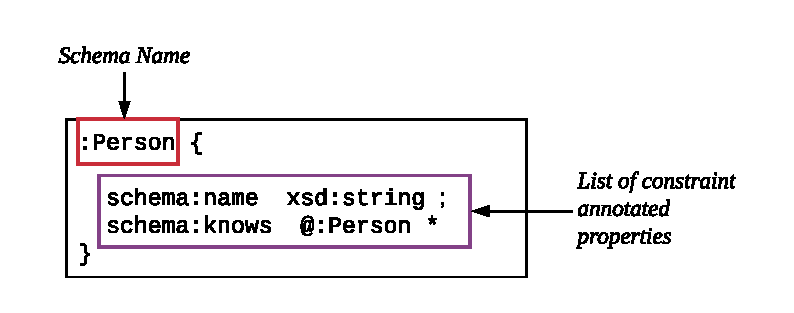
\includegraphics[scale=0.7]{images/shex-example-parts.pdf}
    \centering
    \caption[Shape expression modeling the properties of a Person]{Shape expression modeling the properties of a Person.}
    \label{fig:prop-def-shape-diagram}
\end{figure}

In that shape expression we can see that we have a property that represents the name with type string and the default cardinality \textit{(1)}.
And a second property \texttt{knows} whose type is a reference to another person and has multiple cardinality so it represents a list of people you know.

So we have just seen that a shape, in its reduced grammar is a set of triple expressions made up of the property, the type and the cardinality,
therefore we can formalize that a shape is defined as,

\begin{equation}\label{eq:shape-formalization}
\begin{gathered}
S = \{ (p_{1},t_{1},c_{1}),\ (p_{2},t_{2},c_{2}),\ \dots,\ (p_{n},t_{n},c_{n})\ |\ p \in String,\\
t \in RDF\ Type,\ c \in \{[0,0],\ ...,\ [\infty,\infty] \} \}
\end{gathered}
\end{equation}

where $p \rightarrow property\ name$, $t \rightarrow type$ and $c \rightarrow cardinality$.
And therefore an schema is defined as,

\begin{equation}\label{eq:schema-formalization}
SC = \left \{ S_1,\ S_2,\ \dots,\ S_n \right \}
\end{equation}


% S E C T I O N   P L A I N   O B J E C T S   E X P R E S I V I T Y

\section{Plain Objects Expressivity}
Plain objects can be coded in any object oriented programming language, or at least in
any language that supports this paradigm. First we will explore how plain objects are 
generally coded, then how the language increases or decreases the expressivity and
finally we will generalize the core concepts that can be expressed by any plain object
codification.

\begin{figure}
    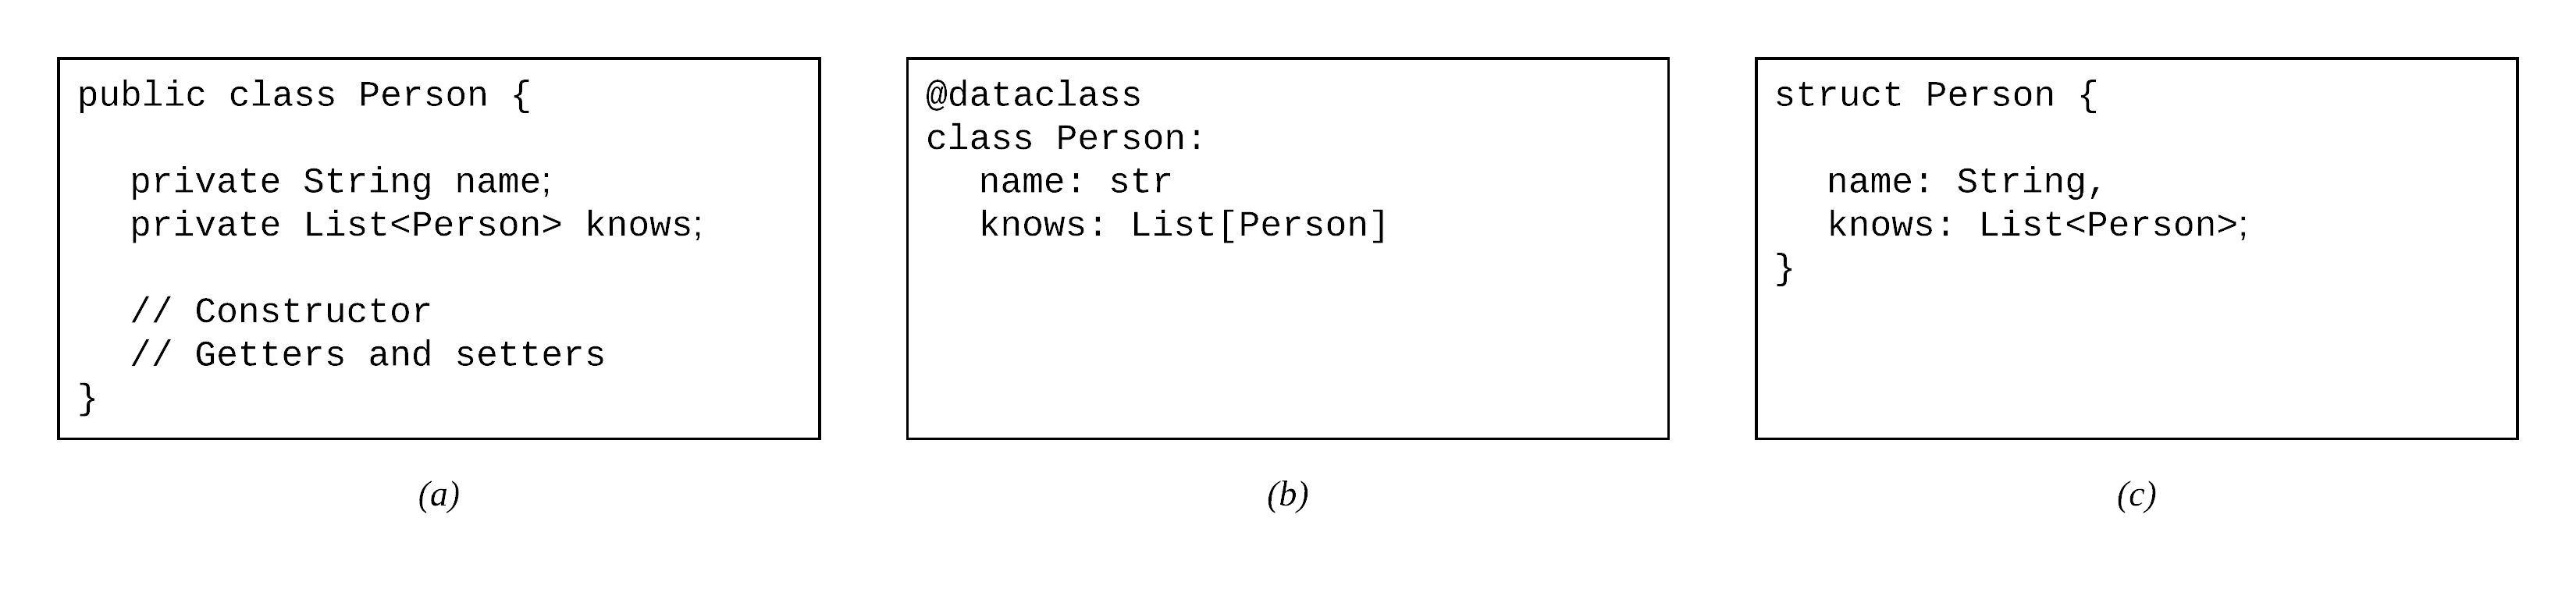
\includegraphics[width=\textwidth]{images/codings-exmaple.png}
    \centering
    \caption[Java, Python and Rust codings of Person object.]{Java, Python and Rust codings of Person object. 
    \textit{a} corresponds to Java, \textit{b} corresponds to Python and \textit{c} corresponds to Rust.}
    \label{fig:person-codings}
\end{figure}


\subsection{Plain Objects Structure}
From the existing programming languages we can infeer the general structure of plain objects. For this porpuse
we take the PYPL Index \textit{(PopularitY of Programming Language)} \footnote{\url{http://pypl.github.io/PYPL.html}}
from June 2020 and take the 2 most used programming languages that support the object oriented paradigm,
those would be Java and Python. And then, just to enlarge the scope we will take Rust because it is a new programming
language that includes lots of features.

\cref{fig:person-codings} shows three models that correspond to the codification of the Person schema from
\cref{fig:shex-translate-small}. For example if we analyze the Java fragment, that seems to be the most complex
one out of the three fragments we can see in \cref{fig:java-analysis} that it is composed by the \textit{Schema Name},
the \textit{List of Type Annotated Properties} and some \textit{Language Specific Code}. This corelates to the other
two programming languages as they also contain this three elements. Therefore after this brief analysis we can generalize that,

\begin{equation}\label{eq:plain-object}
\begin{gathered}
PO = \{ (p_{1}, t_{1}),\ (p_{2}, t_{2}),\ \dots,\ (p_{n}, t_{n})\ |\ p \in String,\\
t\in Language\ Specific\ Type\ System \} + lsc
\end{gathered}
\end{equation}

where $p \rightarrow property\ name$, $t \rightarrow type$ and $lsc \rightarrow language\ specific\ code$.
And therefore a model based on plain objects is defined as,

\begin{equation}\label{eq:plain-object-model}
MO = \{ PO_1,\ PO_2,\ \dots,\ PO_n \}
\end{equation}

where $PO$ represents the plain object.

It is important to note that part of that language-specific code is responsible for representing the language-specific type system.
Therefore, before formalizing our generalization, we must explore whether the type system of a language affects its expressiveness
and, if so, find those types that are common to most languages of this type, if any.

\begin{figure}
    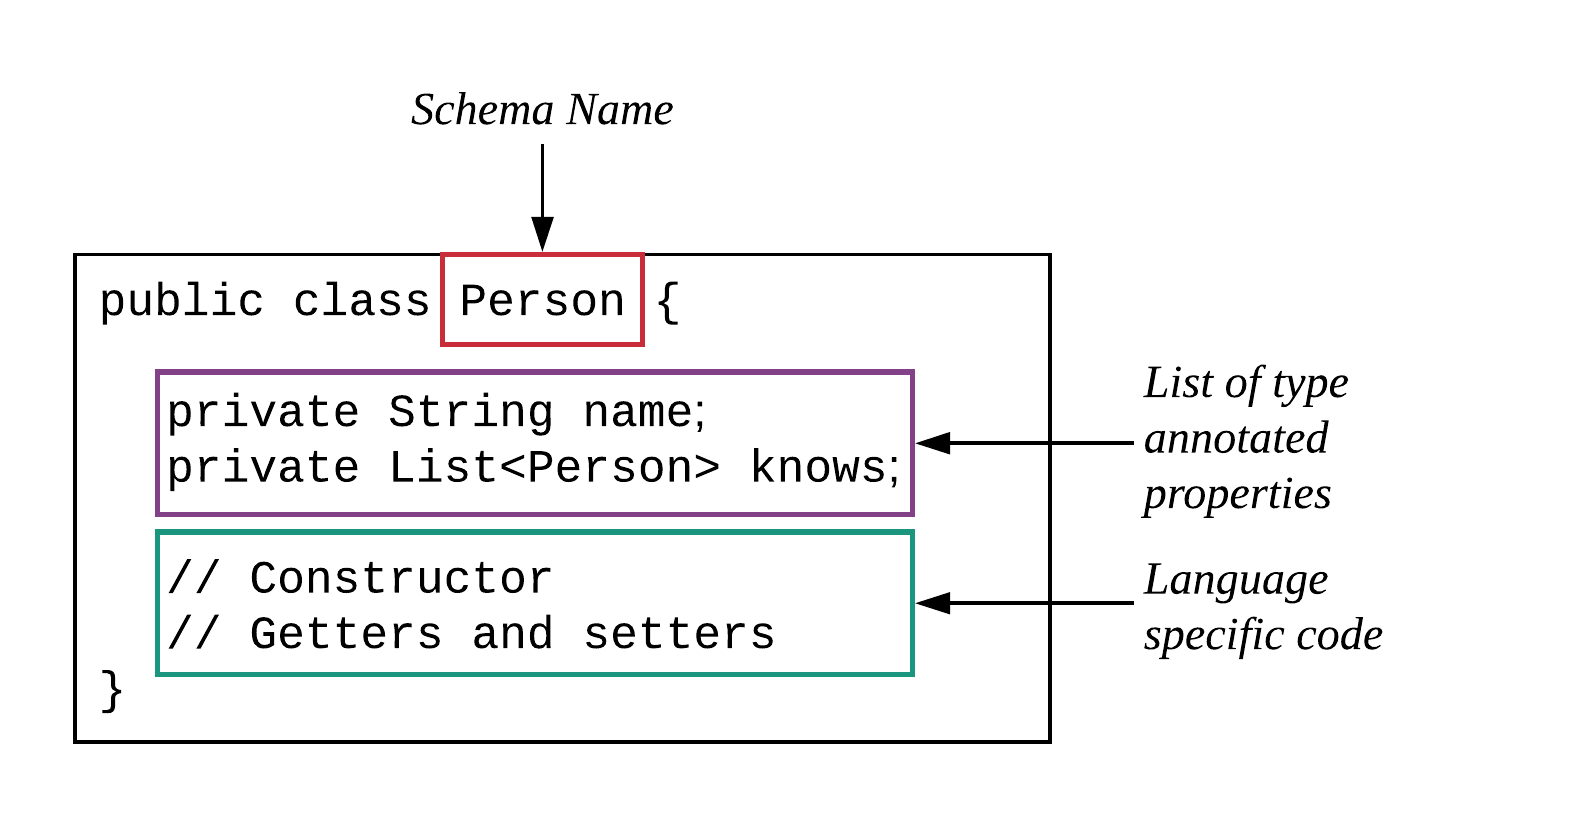
\includegraphics[scale=0.2]{images/java-analysis.png}
    \centering
    \caption[Java plain object decomposition.]{Java plain object decomposition.}
    \label{fig:java-analysis}
\end{figure}

\subsection{Plain Objects Language Expressivity Dependance}
In \cref{fig:person-codings} we can see that all of three languages use similar types to represent the Person model. But with
just one example we cannot generalize that the language does not affect the expressivity of the plain objects. In order to
test that condition and prove that the language affects or doesn't affect the expressivity of plain objects we will need first
to find two \textit{type-independent languages}.

\begin{definition}[Type-independent languages]
    Two languages $L_1$ and $L_2$ are type-independent if and only if one of the languages contains a type that cannot be
    represented by means of a linear combination of any other type of the other language.
\end{definition}

For example, lets take Java \textit{$L_1$} and Rust \textit{$L_2$}, examples \textit{(a)} and \textit{(c)} from \cref{fig:person-codings}.
Rust contains the type $Either<A,B>$, this type allows the type $A$ or $B$ and when accessed is not an $Either$ is either $A$ or $B$. In
Java there is no $Either$ type, and someone can say that we could achive a similar type by using inheritance and classes composition. But
at the end when accessed the type would be the type of the upper class. \textbf{Therefore Java and Rust are type-independent languages}.

Now in order to see if the expressivity depends on the types of a language let's assing values to Java and Rust by using the same
$Either<A,B>$ type. As can be see in \cref{fig:java-rust-comparison} Java does not allow to express the same as Rust is expressing
in this example. And therefore we can conclude that the expresivity of plain object is stronggly related to the build-in types that
the programming language in which they are coded provides.

\begin{center}
	\noindent\begin{minipage}[t]{.4\textwidth}
        \begin{lstlisting}[language=Java,frame=topline,numbers=left,title=\scriptsize{Person Rust Struct},
            basicstyle=\ttfamily\scriptsize]{a}
stuct Person {
    name: String,
    knows: List<Person>,
    owningPet: Either<Dog,Cat>,
}
		\end{lstlisting}
	\end{minipage}\hfill
	\begin{minipage}[t]{.5\textwidth}
        \begin{lstlisting}[language=Java, frame=t,numbers=left,title=\scriptsize{Person Java Object},
            basicstyle=\ttfamily\scriptsize]{b}
// Imports...
public class Person {
    private String name;
    private List<Person> knows;
    private Pet owningPet;
    // Constructor...
    // Getters and Setters...
}
		\end{lstlisting}
	\end{minipage}
    \captionof{figure}{Rust struct modeling a \texttt{Person} to the left.
    And the most similar approximation in Java to te right. In the Java approximation the Pet class is an interface
    that it is inherited by the Cat and Dog classes, that way we allow to store in the variable \texttt{owningPet}
    values of type Cat and Dog.}
	\label{fig:java-rust-comparison}
\end{center}


\subsection{Plain Objects Expressivity Generalization}
In order to obtain a generalization of the plain objects represented by means of object-oriented programming languages,
we will base ourselves on \cref{eq:plain-object} where we defined the composition of a flat object, in this way the
generalization would be as indicated in \cref{fig:po-generalization}. As can be seen this gneralization is not complete
as it does not include the production for the \texttt{type}. Thi is because we have not generalized the type system of the
object oriented programing languages yet.

\begin{figure}
    \begin{lstlisting}[numbers=left,basicstyle=\ttfamily\small]
    plain object     ::= (ID type)+
    \end{lstlisting}
    \caption[Plain Objects Partial Generalization]{Plain Objects Partial Generalization.}
    \label{fig:po-generalization}
\end{figure}

However and motivated not to over-extend the scope of this work instead of extracting a generalization for the possible types
that can be used in each object-oriented programming language, we will try to create this abstraction projecting it on the
most common types used by XML Schema (xsd) \cite{xmlschemasimpleelements}. The main reason is that in RDF, and therefore in ShEx, xsd is the most widely
used type system and the standard of w3c. This leads us to the generalization from \cref{fig:po-generalization-complete} where we re-use the
\texttt{xsd} types and add the \texttt{ID} that actually represents compound types, that is types that are in fact plain objects.

\begin{figure}
    \begin{lstlisting}[numbers=left,basicstyle=\ttfamily\small]
    plain object     ::= (ID type)+
    type             ::= REAL | LIST[type] | STRING | BOOLEAN | ID
    \end{lstlisting}
    \caption[Plain Objects Complete Generalization]{Plain Objects Complete Generalization.}
    \label{fig:po-generalization-complete}
\end{figure}

% S E C T I O N   C O M P A R I S O N 

\section{Shape Expressions and Plain Objects Expressivity Comparison}

Previous section cover the expressivity of Shape Expressions and Plain Objects, in this section we compare both expressivities and
expose if both expresivities are fully compatible or not. In \cref{eq:schema-formalization} we defined an schema and our aim to find if it is possible
to define a function $f$ such that $f(schema)\rightarrow model$ where $model$ is defined in \cref{eq:plain-object-model}. To achieve this function, it
is necessary that the expressiveness of the origin be less than or equal to that of the destination and now that we have already defined the
expressivities of each system we can compare them.

Let's simplify the problem by eliminating all those common factors that we have in both systems. For example, from \cref{eq:schema-formalization} and \cref{eq:plain-object-model}
we have lists of properties with something else, let's reduce the case to having a single property with something else like,
\begin{equation}
\begin{gathered}
\{p,\ t,\ c\ |\ p \in String,\ t \in RDF\ Type,\ c \in \{[0,0],\ ...,\ [\infty,\infty] \}\};\\
\{p,\ t\ |\ p \in String,\ t \in \{String, Real, Boolean, List, Compound\}\}.    
\end{gathered}
\end{equation}
Also in both cases we find that the property is a free text that identifies that property, so we eliminate it from the problem. And we are left with,
\begin{equation}
\begin{gathered}
\{t,\ c\ |\ t \in RDF\ Type,\ c \in \{[0,0],\ ...,\ [\infty,\infty] \}\};\\
\{t\ |\ t \in \{String, Real, Boolean, List, Compound\}\} 
\end{gathered}
\end{equation}
where we need to find if the existis a function $f'$ such that we can map $(t_n,c_n)$ to $(t_n)$.

Now the question changes and what we have to compare is if the $RDF\ Type\ \cap\ \{[0,0],\ ...,\ [\infty,\infty]\}$ can be represented by means of
$\{String, Real, Boolean, List, Compound\}$. For this purpose we will assign different values inside and outside the ranges that we have defined for each set.
In addition, we will define the axiom that the cardinality $(0, \infty)\ \cap\ RDF\ Type$ is the same as $List[RDF\ Type]$. So,
\begin{equation}\label{eq:values-mapping}
    \begin{aligned}
(string,(1,1)) & \rightarrow & (string)\\
(Person,(0,\infty)) & \rightarrow & (List[Person])\\
(string,(1,2)) & \rightarrow & \times \\
(Person,(2,\infty)) & \rightarrow & \times \\
(centimeters,(1,1)) & \rightarrow & \times  
    \end{aligned}
\end{equation}

From the values we gave in \cref{eq:values-mapping} we can see that for some cases there is no schema-object equivalence. However, for others there exist
such and equivalence. Thus, we will define a Subset $S'$ in which we will restrict the types and the cardinality so that those shapes that are defined in
that subset have an equivalent object. Then,

\begin{equation}\label{eq:shape-reduction}
\begin{gathered}
S' = \{ (p_{1},t_{1},c_{1}),\ (p_{2},t_{2},c_{2}),\ \dots,\ (p_{n},t_{n},c_{n})\ |\ p \in String,\\
t \in \{String, Real, Boolean, Compound\},\ c \in \{[1,1],\ [0,\infty] \} \}.
\end{gathered}
\end{equation}

Thus,

\begin{equation}\label{eq:schema-reduction}
\begin{gathered}
SC' = \left \{ S'_1,\ S'_2,\ \dots,\ S'_n \right \}.
\end{gathered}
\end{equation}

That means that we will not be able to translate everything that can be expressed in ShEx Micro Compact Syntax but also means that we will be able
to at least translate some of the shapes. \cref{fig:mapping-f} illustrates this scenario. As you can see in the figure some shapes can be mapped, like the first two,
and other can't, like the third, in this case due to the cardinality not following the \cref{eq:shape-reduction}.

\begin{figure}
    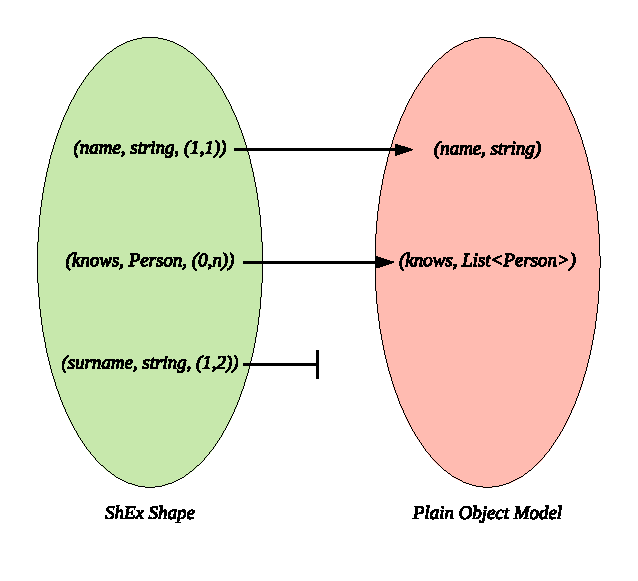
\includegraphics[scale=0.5]{images/shex-lite-mapping.pdf}
    \centering
    \caption[Mapping function from ShEx to Plain Object]{Mapping function from ShEx to Plain Object.}
    \label{fig:mapping-f}
\end{figure}